This section describes the purpose, use, and intended user audience for the Groco product. Groco is a grocery shopping web application that is accessible on PC, smartphones, and tablets. The user of Groco will be able to search for the grocery items and based on the user's preference, the system will suggest the optimal grocery items. The system also allows users to search for recipes, add their recipes and meal plans into their shopping list to perform the optimization and navigation route.

\subsection{Purpose and Use}
The purpose of this product is to help users with grocery shopping. The product can:
\begin{itemize}
    \item look for the item's availability in nearby stores
    \item save money by comparing prices of the item in different stores
    \item save traveling time for shopping by comparing the distance to stores
    \item provide the convenience in planning meals
\end{itemize} 

\subsection{Intended Audience}
The application is a web application and users can access the application from multiple devices. The product is made available publicly and free of charge. The product contains no objectionable material; therefore it is suitable for general grocery shoppers.

\begin{figure}[h!]
	\centering
   	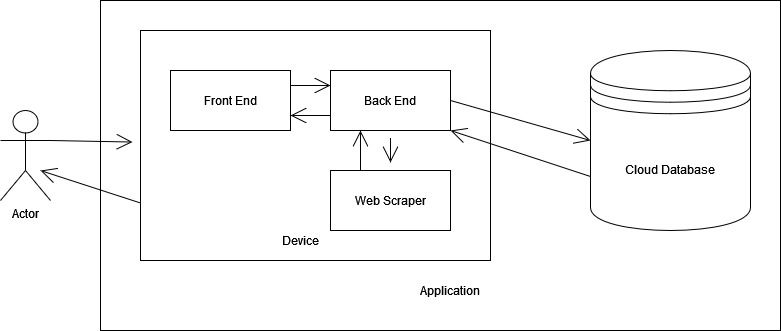
\includegraphics[width=1\textwidth]{images/system_diagram.jpg}
    \caption{High level overview of the system}
\end{figure}
